%\author{D. Crews}

\documentclass[12pt]{article}

\usepackage{amsmath}
\usepackage{graphicx}
\usepackage{bm}
\usepackage{mathabx}
\usepackage[margin=1.0in]{geometry}
\usepackage[english]{babel}
\usepackage{enumitem}
\usepackage{hyperref}
%\usepackage{roman}

\begin{document}
\title{\Large {\bf AA 321 | Aerospace Laboratory\\Lab Eight: Beam bending and vibration}\\[1ex]
  University of Washington}
\date{\today}
\maketitle
%\tableofcontents

\section{Background and objectives}\label{objs}
The deflection and vibration of an airplane wing is very similar to that of a cantilever beam, \textit{i.e.} clamped at one end and free at the other. The same is true of various appendages on spacecraft, such as solar panels and instrument booms. To familiarize yourself with the static and dynamic behavior of cantilever beams several experiments have been performed with instrumented beams. Two beams were tested under static (deflection) and dynamic (vibration) conditions, one steel and the other aluminum.

\subsection{Static deflection: stress determination}
The theory of static deflection of uniform beams is discussed in detail in CEE 220 and AA 331. The purpose of this part of the experiment is to perform strain gauge measurements to compare experimentally determined stress values with the predictions of beam theory for two cantilever beams made of different materials, aluminum and steel. The beams are approximately 63.5 cm long, and their other dimensions are presented in the video.

Each beam is instrumented with a set of strain gauges mounted near the fixed ends, all connected together in such a way as to constitute a Wheatstone bridge (as covered last quarter). The ``push-pull'' connection of the strain gauges is such that their changes in resistance result in an increased unbalance of the bridge, as compared to having only a single strain gauge. There are thus four leads connected to the bridge.\\

\vspace{0.5cm}
The static deflection testing procedure is:
\begin{itemize}[noitemsep]
\item A voltmeter is connected to the bridge leads which is powered with a $5$ V power supply,
\item The ``zero'' voltage of the bridge is measured (that is, voltage at zero load).
\item The beam is loaded by 10, 20, and 30 lbs at $x=40$ and 60 cm from the fixed end.
\end{itemize}

\newpage
The measurements obtained were:
\begin{itemize}[noitemsep]
\item Steel beam, zero voltage -19.36 mV, GF$=2.09$,
  \begin{itemize}[noitemsep]
  \item Load applied at 40 cm,
    \begin{itemize}[noitemsep]
    \item 10 lbs: -18.18 mV
    \item 20 lbs: -17.01 mV
    \item 30 lbs: -15.81 mV
    \end{itemize}
  \item Load applied at 60 cm,
    \begin{itemize}[noitemsep]
    \item 10 lbs: -17.43 mV
    \item 20 lbs: -15.54 mV
    \item 30 lbs: -13.82 mV
    \end{itemize}
  \end{itemize}
\item Aluminum beam, zero voltage 1.793mV, GF$=2.135$,
  \begin{itemize}[noitemsep]
  \item Load applied at 40 cm,
    \begin{itemize}[noitemsep]
    \item 10 lbs: -1.782 mV
    \item 20 lbs: -4.775 mV
    \item 30 lbs: -7.561 mV
    \end{itemize}
  \item Load applied at 60 cm,
    \begin{itemize}[noitemsep]
    \item 10 lbs: -4.073 mV
    \item 20 lbs: -8.653 mV
    \item 30 lbs: -14.009 mV
    \end{itemize}
  \end{itemize}
\end{itemize}

For each dataset, evaluate the stresses and compare with the predictions of beam theory.

\subsection{Dynamic behavior}
The vibrations of a cantilever beam are described in the simplest approximation by the Euler-Bernoulli beam theory (discussed in AA 312). The natural vibration frequencies of a beam are functions of the elastic modulus $E$, the length of the beam $L$, the areal moment of inertia $I$, and the mass per unit length $\rho A$ with $\rho$ mass density and $A$ cross-sectional area. The frequencies (or eigenvalue spectrum) are also dependent on boundary conditions. For a beam fixed at one end and clamped at the other (fixed-free), the Euler-Bernoulli theory predicts the first three spectral modes to be
\begin{equation}
  \omega_1 \approx \frac{3.516}{L^2}\sqrt{\frac{EI}{\rho A}},\quad\quad \omega_2 \approx \frac{22.03}{L^2}\sqrt{\frac{EI}{\rho A}},\quad\quad \omega_3 \approx \frac{61.70}{L^2}\sqrt{\frac{EI}{\rho A}}, \quad\quad \cdots
\end{equation}
and so on, obtained by solving for the eigenvalues using the boundary condition constraint. See the Wikipedia page ``Euler-Bernoulli beam theory'' section ``Example: cantilevered beam'' for a discussion of the corresponding mode shapes.

The apparatus used in this experiment has been designed to test the concept of beam vibration and to introduce some of the experimental methods and techniques used in vibration analysis. A \textit{power spectrum} can be used to determine some of the characteristics of a vibrating system. This is done by measuring the voltage of an accelerometer fixed to the free end of the beam. Four cases are considered, vibration of a steel and an aluminum beam, both with and without an additional mass fixed to the tip of the beam (to introduce an additional frequency and shift the Euler-Bernoulli beam modes). For your analysis, consider,

\begin{itemize}
\item Plot the accelerometer voltage versus time as recorded by the oscilloscope for each data set. Determine the fundamental frequency of vibration by counting the time between successive peaks of the waveform. Can the higher frequencies be observed in this representation (versus time)?
\item Determine the damping coefficient of the fundamental mode using the logarithmic decrement method (be sure to include many cycles of vibration in this estimate rather than using successive peaks).
\item Compute the frequency spectrum of the accelerometer voltage using an FFT. Determine the frequencies of the first three vibrational modes. For the cases without an attached mass, compare to the predicted Euler-Bernoulli frequencies.
\item For two runs ``with mass'', a separate brass weight is attached to the tip of the beam. By comparing the Fourier modes with and without the mass, what effect does the additional weight have on the vibration spectrum? How would one modify the Euler-Bernoulli beam theory to account for the concentrated mass (just conceptually)?
\item The accelerometer has some weight to it as well. Do you expect the presence of the accelerometer to affect the results?
\item Compare the experimental values of frequency to the theoretical values investigated (make a table) and comment on the differences. Also compare the aluminum and steel beam cases and discuss in the context of material properties.
\item Discuss the idea of the time domain vs. the frequency domain (in theory section...).
\end{itemize}

\section{(Optional) A quick introduction to spectral analysis}\label{objs}
A ubiquitously utilized tool in vibration theory is spectral analysis. The main character is the Fourier series, whose central idea is that nearly any periodic waveform\footnote{That is, one satisfying minimally restrictive requirements called the Dirichlet conditions.} $f(x)$ can be decomposed into a series of sine and cosine functions, with convergence in the limit of an infinite number of terms. If the period of $f(x)$ is $L$ (that is, $f(x+L) = f(x)$), then
\begin{equation}
  f(x) = \frac{a_0}{2} + \sum_{n=1}^\infty a_n\cos(k_nx) + b_n\sin(k_nx)\label{fourier}
\end{equation}
is its Fourier series, where the coefficients $a_n$, $b_n$ depend on the particular function $f(x)$ and the frequencies $k_n=\frac{2\pi}{L}n$ are called ``wavenumbers'' (because they tell you the number of wave periods in a length $L$). This works because $\sin(x)$ and $\cos(x)$ form a complete set of orthogonal eigenfunctions for one-dimensional intervals. Let's now go further into this point.
\begin{figure}[h]
  \centering
  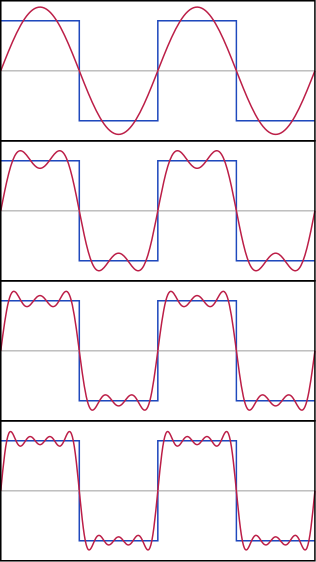
\includegraphics[width=0.19\textwidth]{Fourier/fex}
  \caption{First four partial sums of the Fourier series for the rectangular wave [Wiki].}
\end{figure}

The space that a function lives in is characterized by certain eigenfunctions (\textit{eigen} means ``own'' or ``inherent'', so read as ``characteristic functions'' of the space). The eigenfunctions are a \textit{basis} for the space. In the same way that vector components are found by projection onto basis vectors, a function's components are found by projecting onto the eigenfunctions (Fig. \ref{proj}). Just like basis vectors there are many possible choices of function basis. Of course, the most convenient ones are \textit{orthogonal} and the sines and cosines have just this property.
\begin{figure}[h]
  \centering
  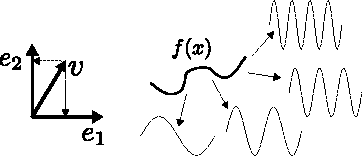
\includegraphics[width=0.75\textwidth]{Fourier/fourier_projection}
  \caption{The Fourier coefficients $a_n$, $b_n$ of $f(x)$ are projections to an orthogonal basis, in the very same way that vector components of $v$ are projections onto basis vectors $e_1$ and $e_2$.}\label{proj}
\end{figure}

What do we mean by orthogonal functions? With vectors, orthogonality means that the measure of one against the other (using the inner product) is zero. For functions the notion of ``measuring one against the other'' is integration over the interval $x\in [0,L]$,
\begin{equation}
  \langle \sin(k_nx)|\sin(k_mx)\rangle = \int_0^L \sin\Big(\frac{2\pi}{L}nx\Big)\sin\Big(\frac{2\pi}{L}mx\Big)dx = \begin{cases} \frac{L}{2} & n=m\\
    0 & n\neq m\end{cases}
\end{equation}
making $\sin(k_nx)$ a family of orthogonal functions. This means that measuring one member against another gives zero, except for itself (try it for $L = 2\pi$ and $n=1$ to convince yourself). Using orthogonality, the coefficients in Eqn. \ref{fourier} are found by the integrals (the projections)
\begin{align}
  a_n &= \frac{2}{L}\int_0^L f(x)\cos(k_nx)dx,\label{f1}\\
  b_n &= \frac{2}{L}\int_0^L f(x)\sin(k_nx)dx.\label{f2}
\end{align}
If the math seems heavy, know that its generally more important to understand what these equations \textit{mean} than to actually do the calculations! There are many tools for calculations.

Now, the set of Fourier coefficients $a_n$, $b_n$ is called the \textit{spectrum} of the function and gives a measure of ``how much'' of the signal is composed of the frequencies $k_n$. For example, if you record yourself playing a note F\# on a guitar (370 Hz) and then calculate the coefficients $a_n$, $b_n$ of the waveform in the music file then there will be a huge peak around 370 Hz. Let's now go into some background on how Matlab will calculate these Fourier coefficients.

\subsection{Complex form of the Fourier series}
Matlab does not calculate the integrals of Eqns. \ref{f1}-\ref{f2}, instead it approximates it using a little fancier theory. One can rewrite the Fourier series in the form
\begin{align}
  f(x) &= \sum_{n=-\infty}^\infty c_ne^{ik_nx},\\
  c_n &= \frac{1}{L}\int_0^Lf(x)e^{-ik_nx}dx\label{fourier2}
\end{align}
by using Euler's identity $e^{ix} = \cos(x) + i\sin(x)$. The notation $\sum_{n=-\infty}^\infty$ means to add all terms in the pairs $n=0, \pm 1, \pm 2, \pm 3, \cdots$. For example,
\begin{equation}
  f(x) = c_0 + c_{-1}e^{-ik_1x} + c_1e^{ik_1x} + c_{-2}e^{-ik_2x} + c_2e^{ik_2x} + \cdots.
\end{equation}
The relationship of these coefficients $c_n$ to the sine and cosine ones is that $c_n = \frac{1}{2}(a_n - ib_n)$ with $+ib$ if $n<0$. This form of the Fourier series is much more economical and the Fourier integral Eqn. \ref{fourier2} is generally easier to calculate than Eqns. \ref{f1}-\ref{f2}. If $f(x)$ is a real function, then all the imaginary parts will cancel out in the summation. Again, understanding what this equation means is more important than doing calculations with it. One is representing $f(x)$ in terms of its orthogonal components, the ``wiggles'' $b_n\sin(k_nx)$ and $a_n\cos(k_nx)$.

\subsection{The ``discrete Fourier transform''}
Suppose you are analyzing a music clip (or beam vibrations) and want to know which frequencies are present. Now the ``Fourier integral'' Eqn. \ref{fourier2} can't be done because the function $f(x)$ is not known. Instead, one has a \textit{time series} of data points, $f = [f_1, f_2, f_3, \cdots, f_N]$ with some sampling rate $\Delta x$. Using this time series, one can approximate Eqn. \ref{fourier2} using the simplest possible integral approximation, just adding up all of the integrand values,
\begin{align}
  c_n = \frac{1}{L}\int_0^Lf(x)e^{-ik_nx}dx \approx \frac{1}{L}\sum_{j=1}^Nf_je^{-ik_nx_j}\Delta x = \frac{\Delta x}{L}\sum_{j=1}^N f_je^{-ik_nx_j}
\end{align}
assuming a constant sampling rate. Because $L = N\Delta x$ and the phase factor simplifies like
\begin{equation}
  -ik_nx_j = -i\frac{2\pi}{L}n\Delta x j = -i\frac{2\pi}{N\Delta x}n\Delta x j = -i2\pi n\frac{j}{N}
\end{equation}
the result, called the discrete Fourier series coefficients, is usually written as
\begin{equation}
  c_n = \frac{1}{N}\sum_{j=1}^Nf_je^{-i2\pi n j/N}\label{fourier3}
\end{equation}
and is simply a summation over the data points with corresponding oscillator functions $e^{ix}$. It is a projection onto the orthogonal basis in the same way as before, just using a discrete set of data points! Now even a summation is pretty slow if the number of terms $N$ is large (like many millions for typical data files). Matlab calculates Eqn. \ref{fourier3} using a clever trick called the \textit{fast Fourier transform} or FFT, which breaks the summation down into smaller chunks. Fortunately, all you have to do is call \texttt{fft(X)} for \texttt{X} your data array!

\subsection{A quick Matlab FFT tutorial}
Here is a quick ``how to'' guide to calculate an FFT in Matlab. Probably the most confusing part is assembling the correct vector of frequencies (note: there is a function in Python that does this for you...!). This example (Fig. \ref{fftex}) reads in a music file (a 9-second clip of a single C chord on the guitar) and analyzes its frequencies.
\begin{figure}[h]
  \centering
  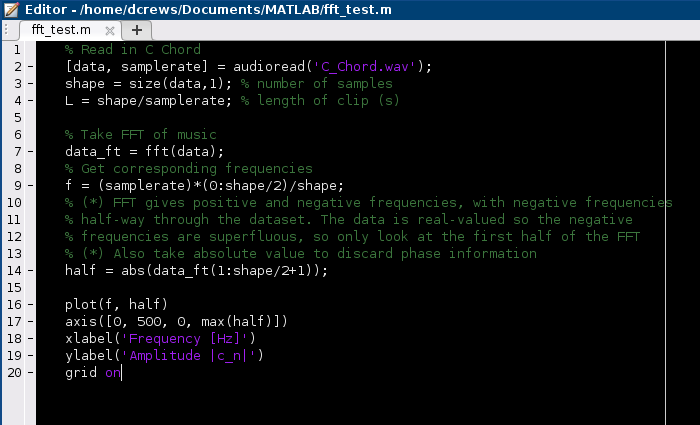
\includegraphics[width=\textwidth]{Fourier/matlab_fft_test}
  \caption{A quick test script to calculate the FFT of a music clip.}\label{fftex}
\end{figure}
To find the sample frequencies, we need to form the wavenumbers $k_n = \frac{2\pi}{L}n$. The FFT calculates the wavenumbers up to a certain cut-off rate called the Nyquist frequency to avoid aliasing effects (which cause the result to look ``pixelly'', so that many video applications use special filters called ``anti-aliasing'' techniques). The Nyquist frequency is half of the sampling rate, so wavenumbers are built up to half of the total samples of the signal. Zooming in on the data with the \texttt{axis} command, Fig. \ref{cchord} is the resulting spectrum of the C-chord. Now try this on your beam vibration data!
\begin{figure}[h]
  \centering
  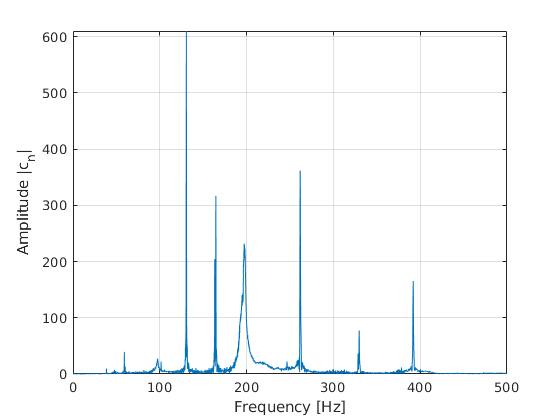
\includegraphics[width=\textwidth]{Fourier/woop}
  \caption{Component frequencies of the C-chord clip. The four notes played were the chord tonic C (131 Hz), then E (165 Hz), G (196 Hz), and finally the octave tonic C (262 Hz). Note that the octave is exactly twice the frequency of the original C! The spike at 393 Hz (G) is a \textit{harmonic} and was not actually played.}\label{cchord}
\end{figure}

% \section{Data reduction and report}
% Be sure to watch the video before your analysis! Please address the following questions:
% \begin{enumerate}[noitemsep]
% \item Calculate the stress value $\sigma_y$ which would exist without a hole.
% \item Calculate the stresses $\sigma_y$ at points 1 and 2 and $\sigma_x$ at point 3 from the measured strains (assume uniaxial stress at these points).
% \item Compare the measured stresses at 1, 2, and 3 with the result of question 1 as well as with the theoretical values predicted for a plate with a hole in it.
% \item From the strain rosette measurements (4-6) determine the magnitudes and directions of the principal stresses $\sigma_1$ and $\sigma_2$ at the center of the rosette. Note the directions of the applied strain gauges.
% \item Determine the magnitudes of the stress components $\sigma_r$, $\sigma_\theta$, and $\tau_{r\theta}$ in the radial and tangential directions at the center of the rosette. Compare the results to the theoretical values and explain any discrepancies. 
% \item How might the accuracy of local stress measurements with strain gauges be improved?
% \item If the yield strength of the specimen be $50000$ psi, what is the maximum load that can be applied before the specimen yields?
% \item How might the stress concentration problem be alleviated?
% \end{enumerate}
% Assume that $E = 10^7$ psi and $\nu = 0.34$ (Poisson ratio) for your calculations.

\end{document}